\documentclass{../source/Experiment}

\major{信息工程}
\name{}
\title{多层神经网络训练}
\stuid{}
\college{信息与电子工程学院}
\date{\today}
\lab{教11-400}
\course{人工智能实验}
\instructor{胡浩基、魏准}
\grades{}
\expname{多层神经网络训练}
\exptype{设计验证}
\partner{}
\begin{document}
\makecover
\section{实验题目}
\subsection{实验6-1}
通过SGD 训练方法 、 ReLu 激活函数 Softmax 最后一层 及 BP 规则 对上述深度神经网络进行训练 并输出训练后的结果 。 为简单起见softmax 函数的导数直接取 1
\subsection{实验6-2}
加入dropout 技巧 ,采用 Sigmoid 激活函数Softmax 最后一层)及 BP 规则,对 上述深度神经网络进行训练,并输出训练后的结果。
\section{实验结果}
\subsection{实验6-1}
预测结果为:
\begin{lstlisting}
            [1,0,0,0,0],
            [0,1,0,0,0],
            [0,0,1,0,0],
            [0,0,0,1,0],
            [0,0,0,0,1]
            \end{lstlisting}
可视化结果:
\begin{figure}[H]
    \centering
    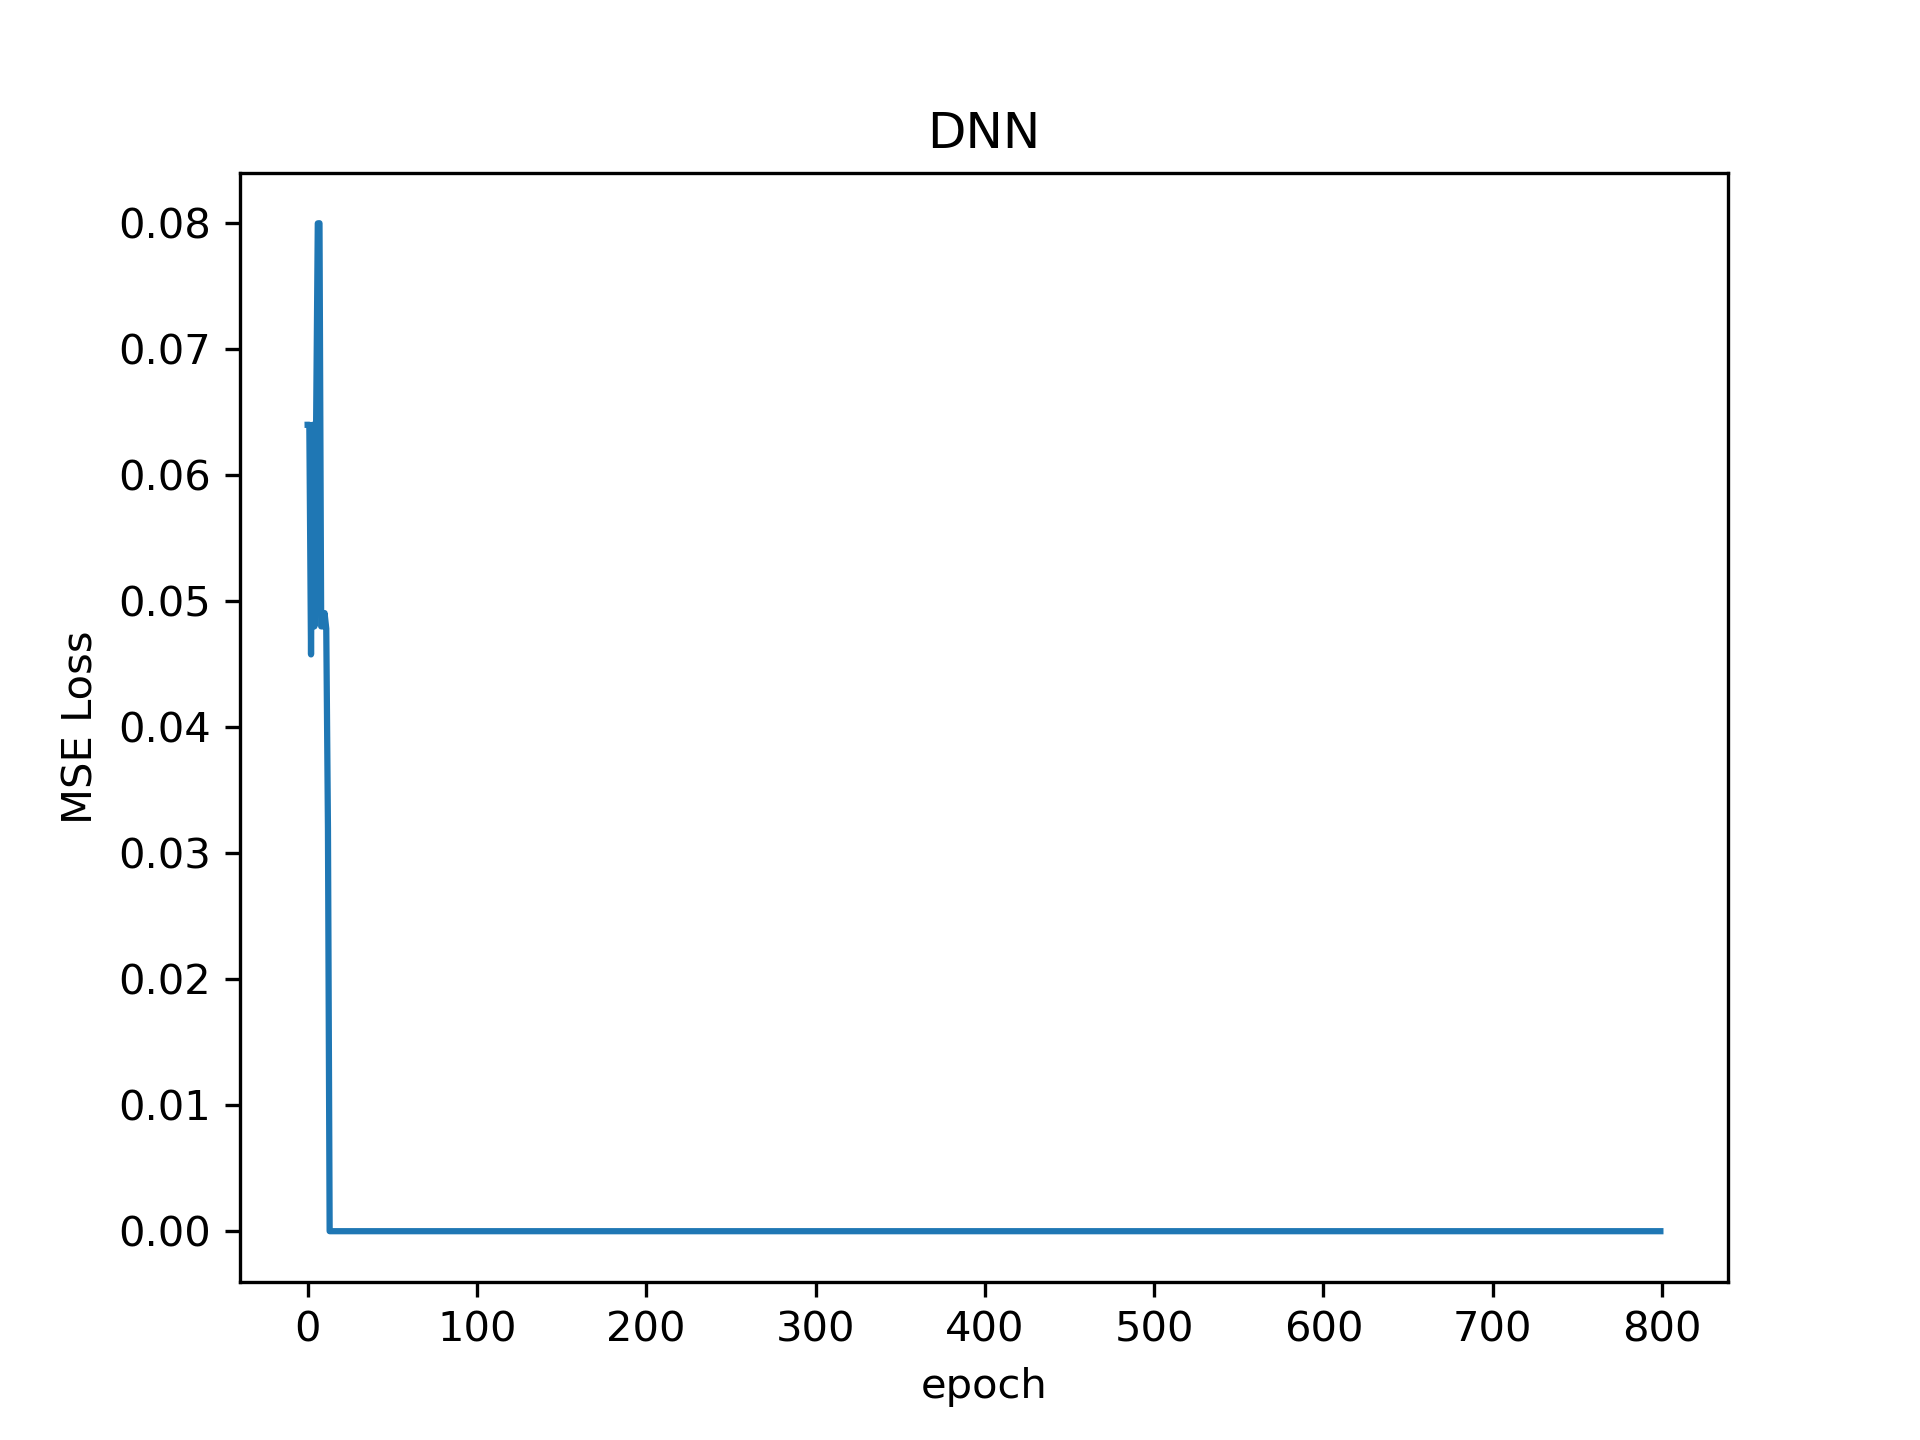
\includegraphics[width = 0.6\textwidth]{Part6/6_1.png}
    \caption{可视化}
\end{figure}
\subsection{实验6-2}
预测结果为:
\begin{lstlisting}

            [0.998  0.     0.     0.002  0.   ]
            [0.     0.998  0.     0.001  0.001]
            [0.003  0.002  0.994  0.     0.001]
            [0. 0.  0. 1.  0.                 ]
            [0.002  0.     0.001  0.     0.997]

            \end{lstlisting}
可视化结果:
\begin{figure}[H]
    \centering
    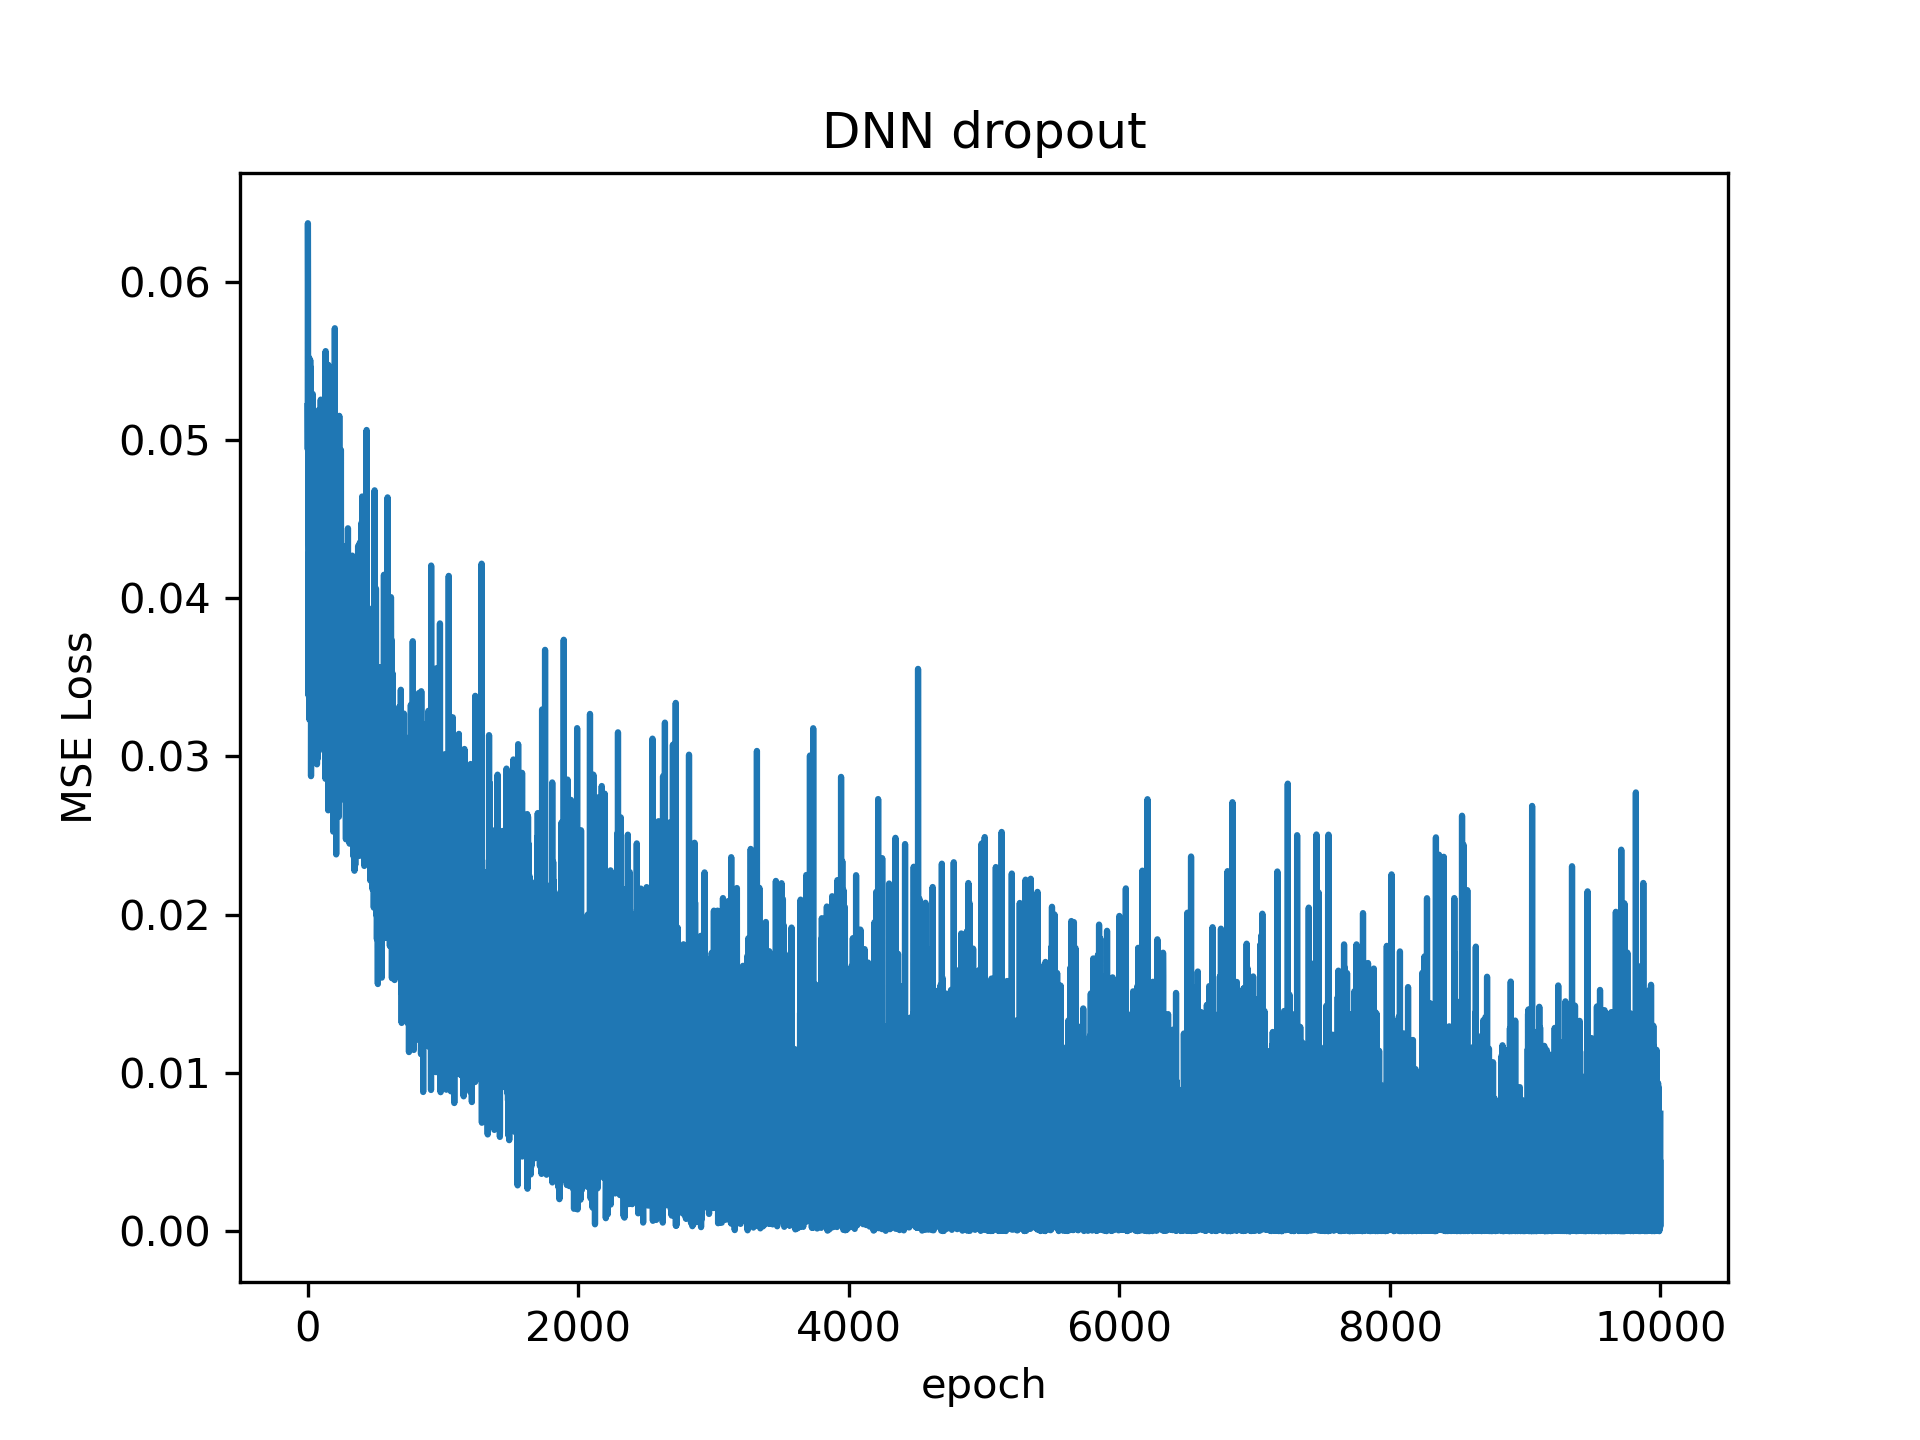
\includegraphics[width = 0.6\textwidth]{Part6/6_2.png}
    \caption{可视化}
\end{figure}

\end{document}


